\chapter{Testing chronosequence predictions with longitudinal data reveals microbial community convergence}
%\chaptermark{Positive frequency-dependence}
%\renewcommand{\sectionmark}[1]{}
\fancyhead[LE, RO]{\thepage}
\fancyhead[RE]{CHAPTER 5}
\fancyhead[LO]{TESTING CHRONOSEQUENCE WITH LONGITUDINAL DATA}
\fancyfoot{}
\renewcommand{\headrulewidth}{0pt}
\setlength{\parindent}{1cm}



\begin{comment}
\documentclass[hidelinks,letterpaper, 11pt]{article}
\usepackage{graphicx, bm, booktabs, lineno, array}
\usepackage[fleqn]{amsmath}
\usepackage{nicefrac}
\usepackage[compress,comma]{natbib}
\usepackage[right=1in, left=1in, top=1in, bottom=1in]{geometry}
\usepackage[parfill]{parskip}
\usepackage[usenames,dvipsnames]{color}
\usepackage[font=large,labelfont=bf,margin=1cm, labelsep = none]{caption} % caption formatting
\usepackage{setspace}
\usepackage{gensymb}
\usepackage{color}
\usepackage{sidecap}
%\usepackage{floatrow}
\usepackage{etoolbox}
\usepackage{tcolorbox}
\usepackage{newpxtext,newpxmath}
\tcbuselibrary{breakable}
%\usepackage{indentfirst}
\newbool{MyRefNumbers}
\usepackage{authblk}
\usepackage{hyperref}
\usepackage{mathpazo}
\usepackage[color=cyan, textsize=tiny]{todonotes}
\usepackage[font={normalsize}]{caption}
\usepackage{adjustbox}
\usepackage{array}
\usepackage{booktabs}
\usepackage{multirow}
\usepackage{tabularx}
% \usepackage{titling}

\setlength{\mathindent}{0pt}
\setlength{\parindent}{1cm}
% \makeatletter
% \makeatother
\pdfminorversion=3

% For table
\newenvironment{myindentpar}[1]%
{\begin{list}{}%
		{\setlength{\leftmargin}{#1}}%
		\item[]%
	}
	{\end{list}}
\newcommand*\samethanks[1][\value{footnote}]{\footnotemark[#1]}
\newcommand\blfootnote[1]{%
	\begingroup
	\renewcommand\thefootnote{}\footnote{#1}%
	\addtocounter{footnote}{-1}%
	\endgroup
}
\newcommand{+}{\raisebox{.4\height}{\scalebox{.6}{+}}}
\newcommand{\minus}{\raisebox{.4\height}{\scalebox{.8}{-}}}
% Command to recount supplement
\newcommand{\beginsupplement}{%
	\setcounter{table}{0}
	\renewcommand{\thetable}{S\arabic{table}}%
	\setcounter{figure}{0}
	\renewcommand{\thefigure}{S\arabic{figure}}%
}
% Command to center oversized images in floats
\newcommand{\centerfloat}{%
	\parindent \z@
	\leftskip \z@ \@plus 1fil \@minus \textwidth
	\rightskip\leftskip
	\parfillskip \z@skip}
\renewcommand\Affilfont{\fontsize{12}{12}\selectfont}
\newcommand{\ignore}[2]{\hspace{0in}#2}
\end{comment}



\begin{comment}
\begin{document}
	
\doublespacing
\title{Testing chronosequence predictions with longitudinal data reveals microbial community convergence}
\author[1, $\dagger$]{Po-Ju Ke}
\author[1, 2]{J. Nicholas Hendershot}
\author[1, $\dagger$]{Tadashi Fukami}
\affil[1]{Department of Biology, Stanford University, Stanford, California, USA}
\affil[2]{Center for Conservation Biology, Stanford University, Stanford, California, USA}
 
\date{\today}
\maketitle
\blfootnote{$\dagger$ Correspondence author: Department of Biology, Stanford University, Stanford, California 94305-5020, USA. Phone: +1 650-721-1711. Fax: +1 650-723-6132. Email: pojuke@stanford.edu, fukamit@stanford.edu}
	
\onehalfspacing
\noindent \textbf{Running title:} Predicting community structure with chronosequence\\
\noindent \textbf{Keywords:} beta diversity, \textit{Carpobrotus edulis}, community assembly, sand dunes, space-for-time substitution, succession\\
\noindent \textbf{Type of article:} Research article
	
\begin{myindentpar}{1cm}
	\textbf{Words in Abstract:} $\sim$ 200\\
	\textbf{Words in main text:} $\sim$ XXX\\
	\textbf{Number of references:} $\sim$ 50\\
	\textbf{Number of figures:} 5\\
\end{myindentpar}
	
\noindent \textbf{Authorship statement:} PJK and TF conceived the study; PJK conducted the study; PJK and JNH analyzed the data; PJK wrote the first draft of the manuscript with substantial contribution from all authors.\\
	
\noindent \textbf{Data accessibility statement:} Should the manuscript be accepted, all data and computer scripts supporting the results will be archived in a public repository, with the DOI included in the article.\\

\linenumbers
\doublespacing
\end{comment}



\section{Abstract}
Chronosequences, defined as a series of sites that differ in the time since their initiation, are commonly used for studying ecological succession, but the usefulness of chronosequences has been controversial. Here, we show how chronosequence inferences can be strengthened by short-term longitudinal data.
Focusing on soil fungi associated with two coastal plants, the ice plant (\textit{Carpobrotus edulis}) and the yellow bush lupine (\textit{Lupinus arboreus}), we characterized fungal communities associated with plant individuals along a plant age chronosequence. 
We then used these data to predict the composition of fungal communities and evaluated the predictions by re-sampling a subset of individuals annually for another two years.
We found that the beta diversity of fungal communities across host plants decreased with plant age. Fungal communities exhibited a consistent compositional shift across the three sampling years, and we were able to predict their composition more accurately as plants aged. Together, the two data types strengthened our inference of a deterministic process shaping the fungal communities. Our results demonstrate how the combination of chronosequence and longitudinal observation can provide a more robust understanding of the processes shaping ecological succession.
\medskip


\noindent \textbf{Keywords:} beta diversity, \textit{Carpobrotus edulis}, community assembly, sand dunes, space-for-time substitution, succession



\section{Introduction}
Ecological communities may converge towards a common structure or diverge because of temporally contingent factors \citep{Fukami2005, DiniAndreote2015, Meiners2015, Clark2019}.
% Predicting successional dynamics has been a central theme of community ecology \citep{DiniAndreote2015, Meiners2015}.
% Classic viewpoint suggests that communities would converge towards a common structure as succession unfolds through time \citep{ConnellSlatyer1977}, whereas recent studies have also highlighted the role of stochasticity and other contingent factors in causing community divergence \citep{DiniAndreote2015, Clark2019}. 
% Nevertheless, elucidating how community trajectories and the underlying mechanisms develop through time remains challenging. 
Predicting which happens in which instances of succession remains challenging because long-term longitudinal data are scarce (but see \citealp{Li2016}), leading to a frequent reliance on chronosequences (i.e., sequences constructed from a series of sites differing in the time since they were formed, \citealp{Walker2010}). 
The utility of chronosequences for inferring community convergence and divergence has been controversial since factors that influence convergence and divergence may change during succession \citep{Johnson2008, Damgaard2019}.
% The assumption of space-for-time substitution behind the chronosequence approach implies that sites of different ages traced the same developmental history.
% However, the utility of chronosequences for inferring temporal dynamics has been questioned, particularly if abiotic and biotic conditions did not remain constant over the time span of the successional change under study \citep{Johnson2008, Damgaard2019}.
One way to strengthen the chronosequence approach is to supplement it with short-term longitudinal data \citep{Damgaard2019}. The assumption that different sites have followed the same history can be tested by repeatedly sampling the chronosequence.
Studies that took this approach showed that chronosequences could accurately predict the temporal changes in ecosystem-level consequences of succession, such as soil formation and biomass accumulation \citep{vanbreugel2006, Lebrijatrejos2010, Walker2010}.
However, it is unclear how accurate chronosequences may be in describing changes in more detailed community structure, such as species composition \citep{Foster2000, Mora2015, Rolo2016}.
% However, when focusing on more detailed community-level properties, such as species richness and community composition, sites that composed the chronosequence may follow different successional trajectories \citep{Foster2000, Mora2015, Rolo2016}. 
% Therefore, when studying whether communities converge or diverge during ecological succession, comprehensive integration of both chronosequence and longitudinal data is necessary for correct inference of the underlying processes.
\par


% Study aims and discuss why soil communities are a great study system
In this study, we combine chronosequence and short-term longitudinal observation to investigate the compositional changes during the succession of plant-associated soil fungal communities.
Using microbial communities to test theories of succession has the advantage that succession occurs at manageable time scales \citep{Fierer2010, Chaparro2013, Gao2019}, therefore allowing the application of our combined approach.
The succession of soil microbial communities, in particular, represents an ideal system to test for community convergence or divergence as plants and other geological processes continuously affect the soil microbial community \citep{BrownJumpponen2014, Castle2016, Dinnage2019}. Although the primary succession of soil microbial communities has been investigated across long time frames of soil development (e.g., \citealp{BrownJumpponen2014, Castle2016}), studies on their fine-scale successional patterns in natural systems are rare. 
\par


% Study approaches
We used a series of high-resolution aerial photos of the coastal dune vegetation at Bodega Bay (California, USA) to construct a chronosequence.
We estimated the age of individual plants and used it as a proxy of the successional stage of their associated soil fungal community. By collecting soil from plant individuals of different ages, and re-sampling a subset of these individuals for another two years, we tested if the two approaches showed similar patterns of community convergence or divergence. For the chronosequence data, we predicted that compositional variation among fungal communities would decrease with the age of their host plant as a result of a deterministic selection force. If the chronosequence correctly captured relevant ecological processes, we should be able to predict the fungal community composition more accurately as plants aged. 
% Our longitudinal data indicated this to be the case.
\par



\section{Methods}
\subsection*{Study system}
% General background of the sytem site
We conducted our field sampling at the coastal foredunes of Bodega Bay, California, USA (38$^{\circ}$19$^\prime$ N, 123$^{\circ}$3$^\prime$ W), located within the Unuversity of California Davis Bodega Marine Reserve and the Sonoma Coast State Beaches. Bodega Bay experiences a Mediterranean-type climate, with an average temperature of 15.8$^{\circ}$C and annual precipitation of 790 mm that occurs mostly between November to April \citep{Conser2009}. 
\par


% General information of the two plants
We focused on the soil fungal community associated with two dominant species at Bodega Bay: ice plant \textit{Carpobrotus edulis} (Aizoaceae) and yellow bush lupine \textit{Lupinus arboreus} (Fabaceae).
\textit{C. edulis} is a south African succulent perennial that was introduced to California for erosion control, but has since invaded California coastal dunes extensively. The plant has a prostrated growth form and, with branches growing over one another, forms thick layers of recalcitrant litter mats up to 40 cm in depth \citep{DAntonio1990}. \textit{C. edulis} alters both biotic \citep{delaPena2010} and abiotic soil properties (e.g., increase soil organic content but decreases soil pH), resulting in growth suppression of other species even after its removal \citep{Conser2009, Novoa2013, Novoa2014}.
\textit{L. arboreus}, is a fast-growing nitrogen-fixing shrub native to central California coastal grassland and dunes. Nitrogen fixation by \textit{L. arboreus} enriches the nutrient-poor sandy soils and facilitates the growth of non-native grasses \citep{Maron1996, Maron2001}. 
\par


%Plant individual selection
We used the age of host plant individuals as a proxy of the successional stage of the soil microbial communities. 
Using a series of aerial photos that were taken annually at Bodega Bay from 1992 to 2016 \citep{Danin1998}, plant ages were estimated by identifying the first year when the individual appeared in the photos. 
We were able to identify individuals to the species level and estimate their age because the foredune vegetation is relatively simple, with low coverage and little vertical structure.
With our age (i.e., successional stage) estimations, we constructed a chronosequence of soil microbial community development at the individual plant level. For the two plant species, we selected 60 individuals from our chronosequence that differed in their age, ranging between 2 to 25 years for \textit{C. edulis} and between 1 to 11 years for \textit{L. arboreus}. 
\par



\subsection*{Soil sampling}
%Soil sampling for microbial community patterns
In July 2015 we collected three soil samples beneath each of the 120 individuals (i.e., 2 species $\times$ 60 individuals). Soil samples were collected roughly on the mid-radius of the plant individual (i.e., midway between the center and the edge of the crown) at three different angles (i.e., azimuth angles 0$^{\circ}$, 120$^{\circ}$, and 240$^{\circ}$). After gently removing the litter that covered the soil surface, we collected soils in separate sterile 50 mL Falcon tubes. 
All soil samples were stored at 4$^{\circ}$C before being processed in the lab. Within one week after collection, each soil sample was passed through a sterile 2 mm mesh sieve, homogenized thoroughly in a sterile plastic bag, and stored at -20$^{\circ}$C. 
The sampling resulted in 360 fungal communities (i.e., 2 species $\times$ 60 individuals $\times$ 3 samples), which were characterized by next-generation sequencing (see section `DNA sequencing of fungal community'). As the fungal communities were collected from plant individuals along the chronosequence, we were able to test for fungal community convergence under the assumption of space-for-time substitution.
\par


To validate the successional dynamics predicted by our samples collected in 2015, we revisited the chronosequence in both July 2016 and 2017 and collected soil samples from a subset of our original plant individuals (i.e., 33 individuals for \textit{C. edulis} and 43 for \textit{L. arboreus}). 
We collected three soil samples from each individual following the same procedure. To avoid being confounded by soil disturbance created during the previous field season, soil samples were collected from positions adjacent to the original sampling position in 2015. 
For each species, we also collected soil samples from three randomly selected juveniles, which were defined as individuals that germinated within one year and were too small to be visible on the aerial photos from the previous year. 
Each year, the  234 soil samples (i.e., 70 individuals $\times$ 3 samples + 2 species $\times$ 3 juveniles) were processed, and their fungal communities were characterized using the same methods as in 2015.
\par



\subsection*{DNA sequencing of fungal community}
We prepared the fungal DNA library for each year's samples with the following steps.
Within one month after sampling, we extracted fungal DNA from all soil samples using the PowerSoil DNA Isolation Kit (Qiagen). 
We amplified the fungal internal transcribed spacer 1 region (ITS1) with primer pair ITS1-F$\textunderscore$KYO1 (5$^\prime$- CTH GGT CAT TTA GAG GAA STA A -3$^\prime$) -- ITS2$\textunderscore$KYO2 (5$^\prime$- TTY RCT RCG TTC TTC ATC -3$^\prime$) \citep{Toju2012}. Primers were concatenated with 3 -- 6-mer Ns \citep{Lundberg2013} and an Illumina sequencing primer region, resulting in a fusion primer for our PCR reactions (forward: 5$^\prime$- TCG TCG GCA GCG TCA GAT GTG TAT AAG AGA CAG -- [3--6-mer Ns] -- [ITS1-F$\textunderscore$KYO1] -3$^\prime$; reverse: 5$^\prime$- GTC TCG TGG GCT CGG AGA TGT GTA TAA GAG ACA G -- [3--6-mer Ns] -- [ITS2$\textunderscore$KYO2] -3$^\prime$). 
Our PCR reaction consisted of 3.2 $\mu$L of MQ water, 5 $\mu$L of MyTaq HS DNA polymerase Mastermix (Bioline), 0.4 $\mu$L of each primer (10$\mu$M for both forward and reverse primer), and 1 $\mu$L of extracted DNA (total volume 10 $\mu$L). PCR reactions were run with a hot start at 95$^{\circ}$C for 2 min, followed by 36 cycles of 95$^{\circ}$C for 20 sec, 50$^{\circ}$C for 20 sec, 72$^{\circ}$C for 50 sec, and a final extension at 72$^{\circ}$C for 10 min. We set a 1$^{\circ}$C/s ramp rate to prevent chimeric amplicon generation. 
After this first PCR process, a subsequent second PCR was run to add sample-specific tags. The fusion primers used in this second PCR concatenates P5/P7 Illumina adaptors, 8-mer index sequences, and the sequencing adaptor \citep{Hamady2008} (forward: 5$^\prime$- AAT GAT ACG GCG ACC ACC GAG ATC TAC AC -- [8-mer tag] -- TCG TCG GCA GCG TC -3$^\prime$; reverse: 5$^\prime$- CAA GCA GAA GAC GGC ATA CGA GAT -- [8-mer tag] -- GTC TCG TGG GCT CGG -3$^\prime$). The second PCR consisted of 8 cycles with the same temperature profile as our first PCR but with an annealing temperature of 50$^{\circ}$C. 
After PCR, we purified the product using the AMPure XP Kit (Agencourt), with a sample : bead ratio of 1 : 0.6. Finally, we pooled 5$\mu$L of normalized PCR product from each sample to create a pooled library for samples collected at that year. 
Libraries were stored at -80$^{\circ}$C and later pulled together based on their Qubit reads after the library for 2017 samples was prepared in November 2017.
The final pooled library, consisting of fungal DNA from samples collected across all three years, was sequenced using the Illumina MiSeq sequencer of the Stanford Functional Genomics Facility (2 $\times$ 250 cycle sequencing kit) with 15$\%$ PhiX spike-in.
\par


We processed the Illumina MiSeq sequencing reads with the Claident pipeline (\citealp{Tanabe2013}, v0.2.2015.11.19). We converted raw Miseq BCL data to FASTQ data with the program bcl2fastq v1.8.4. We then demultiplexed the library based on the sample-specific 8-mer index sequences. All sequencing reads with low quality (i.e., sequencing quality scores $<$ 30) were deleted. The obtained forward and reverse sequencing reads were fused using PEAR v0.9.6 \citep{Zhang2014}, and low-quality merged reads (quality score $<$ 30 or length $<$ 150 bp) and chimeric reads were eliminated using UCHIME v4.2 \citep{Edgar2011}. Sequencing reads that passed through all filtering processes were then clustered into operational taxonomic units (OTUs), based on a 97$\%$ sequence similarity cutoff, using VSEARCH \citep{Rognes2016}. After clustering, fungal OTUs with less than ten total sequencing reads were removed, resulting in a final sample $\times$ OTU matrix. Taxonomy was assigned to the OTUs using the RDP Naive Bayesian rRNA Classifier v2.11 \citep{Wang2007} trained on the Warcup Fungal ITS training set 2 \citep{Deshpande2016} for fungi. Based on the taxonomic assignment results, ITS1 sequences other than those of the Kingdom Fungi were removed from the dataset, and the remaining OTUs with sufficient taxonomic information were assigned a trophic mode based on \textit{FUNGuild} \citep{Nguyen2016}.
% Potential contaminant OTUs were identified statistically based on their prevalence in PCR and extraction negative controls (two of each for every 96 well plate reaction) using the R package decontam \citep{Davis2018}.This resulted in the elimination of \ignore{36} XX fungal OTUs. 
% The whole bioinformatics process resulted in \ignore{19,868} XX,XXX OTUs, representing \ignore{1,772,220} X,XXX,XXX ITS1 sequencing reads. 
\par



\subsection*{Data analysis}
% General overview of data analysis and data processing
% We applied both distance-based and model-based analyses to test for convergence of fungal communities during succession.
% As our model-based analysis are based on hierarchical Bayesian approaches (see below, \citep{Ovaskainen2017}), we fitted models by treating each soil sample as separate observation units. On the other hand, we summed the OTU abundances of the three samples that were collected from the same plant individual during the same year to avoid pseudo-replication in the distance-based analysis (i.e., treating plant individuals collected at different years as observation units). 
We summed the OTU abundances of the three samples that were collected from the same plant individual during the same year to avoid pseudo-replication (i.e., treating plant individuals collected at different years as observation units). Individuals that recovered less than three samples from the sequencing run were removed from the following analysis. 
The sample $\times$ OTU table was then rarefied to 1000 sequencing reads per sample (R package phyloseq, \citealp{McMurdie2013}). 
For the following analysis, we focused on fungal OTUs that occurred in more than 20$\%$ of the samples in order to ensure adequate model fit in our model-based analysis (see later for detail). 
% For consistency, the same 20$\%$ frequency constraint was also applied to the distance-based analysis. 
Note that all statistics with plant age as a predictor were performed separately for \textit{C. edulis} and \textit{L. arboreus}. This is because the two species vary in their longevity and thus the same age does not necessarily represent the same life stage.
\par


% Distance-based approach -- NMDS
We first applied a distance-based approach to characterize the overall differences in fungal community composition among plant individuals at different sampling year. 
To visualize the compositional shifts, we further limited our ordination to plant individuals that were sampled at all three years (i.e., age $\tau$, $\tau + 1$, and $\tau + 2$ in 2015, 2016, and 2017, respectively). 
We visualized fungal communities of the remaining 90 \textit{C. edulis} and 120 \textit{L. arboreus} observation units (i.e., plant individual $\times$ year sampled) with non-metric multidimensional scaling (NMDS) based on Bray--Curtis dissimilarity (with R package vegan). We tested for the effects of soil host species identity and plant age with permutational multivariate analysis of variance (PERMANOVA with 999 permutations, \citealp{Anderson2011}). 
On the NMDS plot, we used a vector to connect fungal communities that were collected from the same individual during different sampling years, pointing from the coordinates that represented the 2015 fungal community to that of 2016 and 2017. We quantified the x- and y-components of the vector (i.e., $\Delta$NMDS 1 and $\Delta$NMDS 2), which represent the overall direction and magnitude of community shifts. In particular, vectors that moved toward similar direction indicate a consistent compositional shift of fungal communities over succession.
\par


% Distance-based approach -- Spatial beta
Fungal communities collected along the chronosequence allowed us to test for community convergence based on the assumption of space-for-time substitution. Namely, if fungal communities were converging over succession, the dissimilarity among fungal communities associated with different plant individuals would decrease with the age of their host plant. 
For each species, we used the data from all 60 plant individuals collected in 2015 and calculated the beta diversity among fungal communities associated with plant individuals of the same age class. Beta diversity for each age class was calculated as the distance of fungal communities to the centroid of each age class.
% We also calculated beta deviation following \citep{Tello2015, Vannette2017}. The purpose is to compare the observed level of beta diversity in each age class to those expected if communities were assembled randomly within the constraints imposed by the observed species abundance distributions.
We then fitted linear models to quantify how beta diversity varied with increasing plant age.
As beta diversity was not meaningful for age classes with only one individual (i.e., distance to centroid within the age class would be zero), we deleted these communities when fitting linear models. 
We also visualized the trend in beta diversity with increasing plant individual age with a three-year moving window (i.e., the centroid was calculated using fungal communities associated with age $\tau - 1$, $\tau$, and $\tau + 1$ individuals).
\par


% Model-based approach -- HMSC
We also tested for community convergence using the re-sampling data that we collected in 2016 and 2017 via repeatedly sampling a subset of the plant individuals. 
For this analysis, we turned to a model-based approach with the R package HMSC \citep{Ovaskainen2017}, which is able to capture OTU-specific temporal patterns and generate predictions of the community composition. 
% Different from the previous ordination approaches, this model fitting were performed by treating each soil sample as separate observation units in order to take advantage of the hierarchical Bayesian approach implemented in \textit{HMSC} \citep{Ovaskainen2017}. 
To predict fungal OTU abundances, we fitted models with plant age as fixed effect and plant individual as random effect on a training set, which consisted of data from all 60 plant individuals collected in 2015. The abundance of fungal OTUs were assumed to follow an over-dispersed Poisson distribution to account for changes in the mean--variance relationship inherent with microbial count data. For all models, the MCMC sampling was conducted for 1,000,000 iterations, with a burn-in phase of 500,000 iterations and thinned every 100 iterations. 
After fitting the model, we used data collected from 2016 and 2017 as separate test sets to see if the predictability of fungal communities varied with plant age. 
In particular, we quantified the Bray--Curtis dissimilarity between the predicted and observed fungal community composition (i.e., age $\tau + 1$ and $\tau + 2$ in 2016 and 2017, respectively) and then assessed its relationship with plant age by fitting linear models. 
% The relationship between the Bray--Curtis dissimilarity and plant age in 2015 (i.e., age $\tau$) was assessed with the R package glmmTMB, assuming that the dissimilarity metric followed a beta distribution). If dissimilarities decreased with plant age, we would conclude that the communities are converging over succession since the predictability of the fungal community composition increased. 
If the Bray--Curtis dissimilarity decreased with plant age, we concluded that the communities are converging over succession since the predictability of the fungal community composition increased. 
% To assess the robustness of the community convergence pattern, we also fitted additional models for common OTUs (i.e., those that occurred in more than 50$\%$ of the samples) and at different taxonomic resolution (i.e., by aggregating OTUs based on assigned taxonomy, ranging from Phylum to Genus).
\par



\section{Results}
% Distance-based approach -- NMDS
Fungal composition changed across the three sampling years, mainly captured by the NMDS 2 axis, whereas the effect of host species was represented by the NMDS 1 axis (Fig.~\ref{fig:3YrNMDS_Individual}; PERMANOVA, species effect: $R^{2}=0.13$; age effect for \textit{C. edulis}: $R^{2}=0.06$; \textit{L. arboreus}: $R^{2}=0.05$; age effects were tested separately for the two species; all $P<0.001$).  
Most fungal communities exhibited a consistent compositional shift across the three sampling years. Fungal communities associated with the same individual showed an upward movement along the NMDS 2 axis, but inconsistent movement in NMDS 1 (Figs.~\ref{fig:FourQuadrate_Individual_Species} and \ref{fig:FourQuadrate_Individual_Species_SI}).
The yearly compositional shifts were larger for \textit{L. arboreus} compared to \textit{C. edulis}, as indicated by the ellipses in Figure~\ref{fig:3YrNMDS_Individual} and the higher proportion of upward movement in Figure~\ref{fig:FourQuadrate_Individual_Species}.
% See also Figs.~\ref{fig:3YrNMDS_Sample} and \ref{fig:FourQuadrate_Sample_Species} for similar patterns when separate soil samples, instead of plant individuals, were plotted as units of replication.
\par


% Distance-based approach -- Spatial beta
For fungal communities collected from plant individuals along the chronosequence in 2015, beta diversity declined significantly with plant age for both \textit{C. edulis} and \textit{L. arboreus} (Fig.~\ref{fig:CombinedFull2015Beta_Individual_SI}; \textit{C. edulis}: Pearson's $r=-0.46$, $P=0.001$; \textit{L. arboreus}:  Pearson's $r=-0.27$, $P=0.04$). Similar trend in beta diversity were observed with a three-year moving window average (Fig.~\ref{fig:CombinedFull2015Beta_Individual}).
% However, only the beta deviation of \textit{C. edulis} decreased with plant age (Fig.~\ref{fig:Full2015Beta_Individual}b). 
% See also Figs.~\ref{fig:Full2015Beta_Sample} and \ref{fig:MovingWindowBeta_Sample} for similar patterns when soil samples were plotted as units of replication.
\par


% Model-based approach -- HMSC
Bray--Curtis dissimilarity between the model prediction and observed community composition decreased (Figs.~\ref{fig:HMSC_Species_Individual_Full2015} and \ref{fig:HMSC_Species_Individual_Full2015_SI}; all $P<0.01$), indicating convergence in fungal species composition.
Test sets collected in both 2016 (Fig.~\ref{fig:HMSC_Species_Individual_Full2015}) and 2017 (Fig.~\ref{fig:HMSC_Species_Individual_Full2015_SI}) showed the same convergence pattern (Pearson's $r$ for \textit{C. edulis} in 2016 and 2017: $-0.55$ and $-0.64$; for \textit{L. arboreus} in 2016 and 2017: $-0.36$ and $r=-0.40$; all $P < 0.05$). 
% The results were robust when we fitted models with different fungal taxonomic levels and frequency thresholds.
When inspecting the changes in fungal trophic mode (Fig.~\ref{fig:Funguild_HMSC_Species_Individual_Full2015}), we found that OTUs within a trophic mode exhibited different temporal trends. Moreover, many \textit{L. arboreus}-associated pathotrophic fungi increased significantly through time, whereas those associated with \textit{C. edulis} mostly decreased or increased less significantly (Fig.~\ref{fig:Funguild_HMSC_Species_Individual_Full2015Pathogen}).
% See also Fig.~\ref{fig:HMSC_Species_Sample_Full2015} for similar patterns when plant individuals were plotted as units of replication. 
\par



\section{Discussion}
% Biology of the system -- plant host effects and who's changing? 
By repeatedly sampling the soil fungal community along a chronosequence of soil conditioning by plant individuals, we found multiple pieces of evidence for community convergence (Figs.~\ref{fig:FourQuadrate_Individual_Species}--\ref{fig:HMSC_Species_Individual_Full2015}).
At our field site, plant-associated soil fungal communities started to assemble as plants colonize bare sand. 
The plant species that arrived and conditioned the soil affected fungal community assembly, selecting for different species over time (Fig.~\ref{fig:3YrNMDS_Individual}). These results indicate that host plants drove the succession of the fungal communities \citep{RoyBolduc2016, Scheublin2004}.
This pattern contrasts with previous studies that showed little effect of plant species identity on the primary succession of soil microbes \citep{BrownJumpponen2014, Sikes2014}.
With our model-based approach, we found that the abundance of many pathotrophic fungi increased through time when associated with \textit{L. arboreus}, whereas pathotrophic fungi associated with \textit{C. edulis} either decreased or increased to a lesser extent (Fig.~\ref{fig:Funguild_HMSC_Species_Individual_Full2015Pathogen}).
This result might indicate a release from soil-borne enemies of the introduced \textit{C. edulis} \citep{Keane2002, Callaway2004b}, and that pathotrophic fungi at Bodega Bay are better at forming associations with the native \textit{L. arboreus}.
\par


% Biology of the system -- why are they changing? 
Past studies showed that the two plant species in our study have large effects on the soil abiotic environment.
\textit{C. edulis} produces a thick recalcitrant litter mat that increases soil organic content and decreases soil pH \citep{Novoa2013, Novoa2014}, whereas \textit{L. arboreus} increases soil nitrogen levels \citep{Maron1996, Maron2001}. 
It seems likely that the conditioning effects imposed by host plants increase as plants aged, causing fungal community convergence \citep{Dinnage2019}. 
Fungal communities associated with \textit{L. arboreus} showed larger and more consistent compositional shifts throughout the three years compared to communities associated with \textit{C. edulis} (Figs.~\ref{fig:3YrNMDS_Individual} and \ref{fig:FourQuadrate_Individual_Species}). 
One potential explanation is that \textit{L. arboreus} imposes stronger selection through their nitrogen-fixing activity, modifying the nitrogen-fixing bacterial community and consequently causing different fungal--bacterial interactions \citep{Johansson2004}.
In addition, three years represent a longer proportion of the life span of \textit{L. arboreus} individuals compared to \textit{C. edulis} (i.e., maximum 11 years for \textit{L. arboreus}, but more than 25 years for \textit{C. edulis}), which might be another reason explaining the more consistent compositional shift for \textit{L. aboreus}. 
\par


% Comments on the integrated approach -- Spatial and temporal data
Studies supporting community convergence are usually based on one of the two types of data. Chronosequence data, i.e., observational data based on space-for-time substitution, would indicate community convergence if the variation among communities of the same successional stage was smaller for late successional communities (Figs.~\ref{fig:CombinedFull2015Beta_Individual} and \ref{fig:CombinedFull2015Beta_Individual_SI}; see also \citealp{BrownJumpponen2014, Castle2016, RoyBolduc2016}).
Although less common, evidence for convergence has also come from longitudinal data, i.e., temporal data collected by repeatedly sampling the same community throughout succession (e.g., \citealp{Fukami2005, Li2016, Gao2019}).
% Given the critiques against the chronosequence approach \citep{Johnson2008} and the logistical challenges of collecting long-term longitudinal data, studies have applied an integrated approach by supplementing the chronosequence pattern with repeated sampling. 
Here, we combined the two types of data and found that they both indicated convergence (Figs.~\ref{fig:CombinedFull2015Beta_Individual} and \ref{fig:HMSC_Species_Individual_Full2015}). 
Past studies that used this combined approach have shown that the validity of chronosequences depends on the system or community characteristic being tested \citep{Foster2000, Clark2019}.
At the coastal dunes undergoing primary succession, the agreement between the two data types strengthened our inference of an underlying deterministic process shaping soil fungal communities. 
\par


% Comments on the integrated approach -- past examples of integrated approaches
When comparing different data types, most studies only qualitatively compared the predicted and observed changes in community structures with correlation analysis (e.g., \citealp{Foster2000, vanbreugel2006, Lebrijatrejos2010}). In addition, studies on community compositional shifts typically focus on the responses of the whole community (e.g., comparing changes of the ordination coordinates of dimension reduction methods).  
Here, we applied a training set--test set approach and quantified the predictability of fungal community composition (see also \citealp{Mora2015}). 
By fitting joint distribution models \citep{Ovaskainen2017} we captured the various responses of fungal OTUs within the community, with temporal patterns differing in their direction and magnitude (Fig.~\ref{fig:Funguild_HMSC_Species_Individual_Full2015}). 
Moreover, as we fitted models to the whole chronosequence data, our predictions reflect the general patterns of OTU abundances without being confounded by noise between consecutive years.
The model-based approach used here thus provided a unique way to examine succession: communities are converging (or diverging) if the predictability increases (or decreases) over time (Figs.~\ref{fig:HMSC_Species_Individual_Full2015} and \ref{fig:HMSC_Species_Individual_Full2015_SI}).
\par


% Comments on the integrated approach -- final conclusions
Although chronosequences have been an essential tool for studying succession, a common perspective is that they are less desirable compared to longitudinal data \citep{Johnson2008}. 
We argue that the two types of data provide complementary insights: chronosequence data can demonstrate that the community changes indicated by the longitudinal data operated across all years, instead of just the period of the longitudinal observation. Thus, the agreement between the two data types allows one to generalize the results to a larger spatial-temporal scale.
We suggest that this combined approach can contribute to more robust understanding of community convergence and divergence in many systems.
% By demonstrating the utility of this integrated approach, we call for more studies combining chronosequence and longitudinal data to provide a more robust understanding of the processes shaping ecological succession.
\par



\section{Acknowledgments}
We thank Kitty Brown, Jackie Sones, and Brendan O'Neil for logistic support at the Bodega Marine Laboratory and Sonoma State Park; Manpreet Dhami and Nora Dunkirk for their assistance with sequencing; Hirokazu Toju for providing bioinformatics scripts; Nancy Chang, Suchana Costa, Marion Donald, Jasmine Gilliam, Ben LeRoy, Michelle Li, Kaoru Tsuji, and Anna Verwillow for field and lab work assistance; Peter Adler, Erin Mordecai, Kabir Peay, and members of the community ecology group at Stanford University for comments.



%\clearpage
%\bibliographystyle{ecollet.bst}
%\bibliography{libraryfixed-abbrev}



\newpage
\section{Figures}
\begin{figure}[h]
	\centering
	\makebox[\textwidth][c]{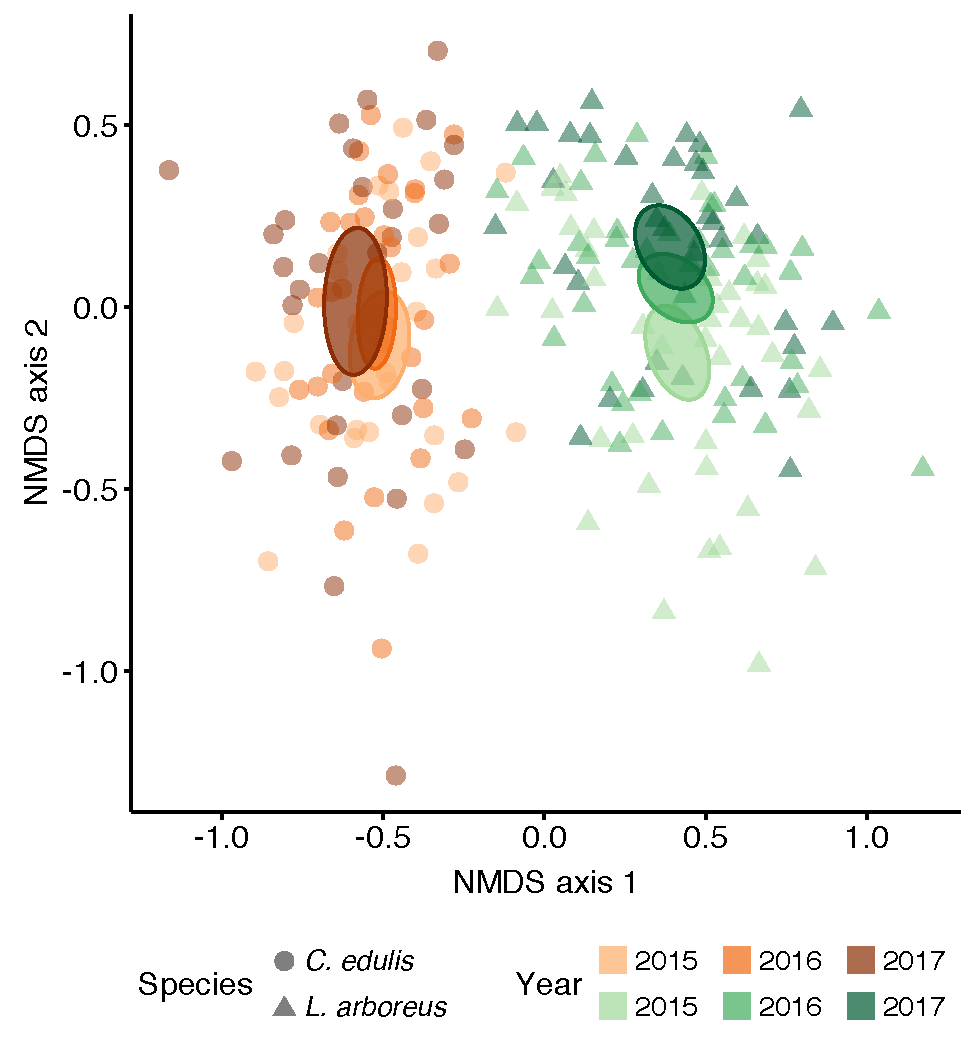
\includegraphics[width=11cm]{Chapter5/3YrNMDS_Species_Common.pdf}}
	\caption[Compositional differences among fungal communities associated with plant individuals across three sampling years.]
		{\hspace{1mm} Compositional differences among fungal communities associated with plant individuals across three sampling years. Each point represents the fungal community of one plant individual. Point shapes represent plant species (circle: \textit{C. edulis}; triangle: \textit{L. arboreus}) and the brightness of colors represent the year of sampling (light orange/green: 2015; orange/green: 2016; dark orange/green: 2017). Ellipses capture the dispersion based on the standard error of the average of all points that were collected from the same species during the same year. 
		% See Fig.~\ref{fig:3YrNMDS_Sample} for identical pattern when soil samples, instead of plant individuals, were plotted as observation units.
		}
	\label{fig:3YrNMDS_Individual}
\end{figure}



\clearpage
\begin{figure}[h]
	\centering
	\makebox[\textwidth][c]{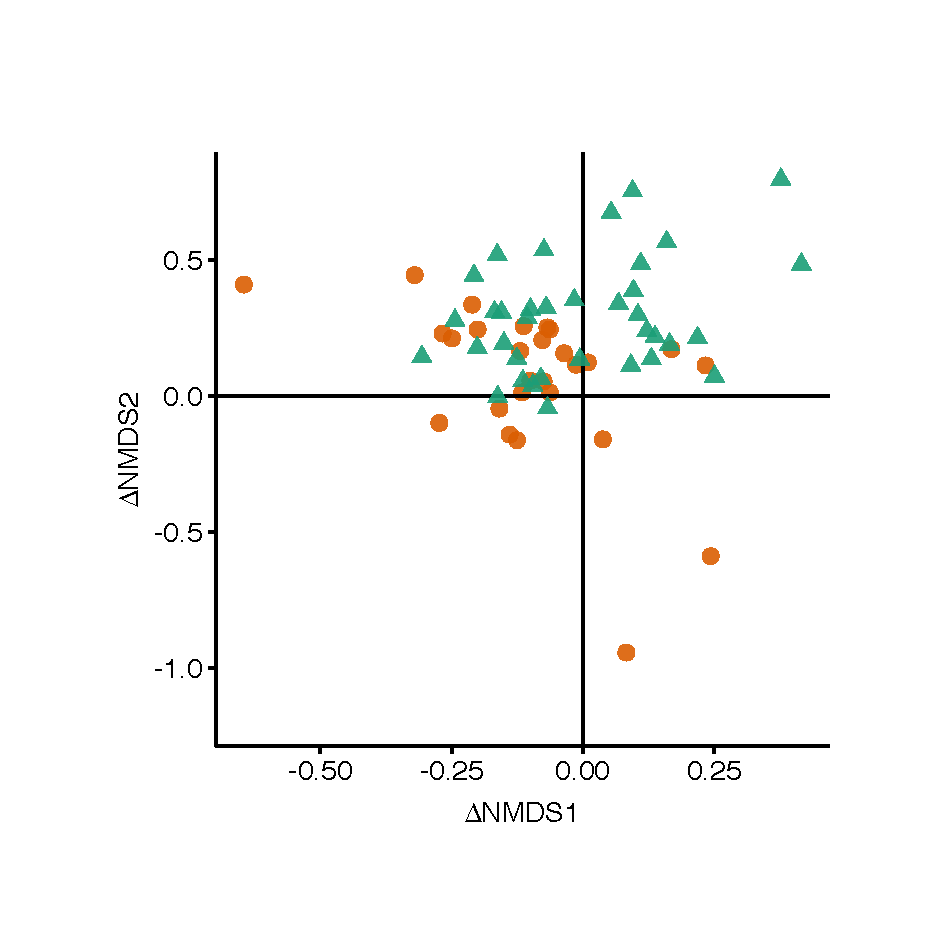
\includegraphics[width=12cm]{Chapter5/FourQuadrateMovement_Species_Common_RevisedMS.pdf}}
	\caption[Overall compositional shifts of the fungal community from 2015 to 2017.]
		{\hspace{1mm} Overall compositional shifts of the fungal community from 2015 to 2017. Each point represent the movement (i.e., x- and y-component of the arrow) of the fungal community associated with one plant individual. A positive x-component (i.e., $\Delta$NMDS 1 $ > 0$) and y-component (i.e., $\Delta$NMDS 2 $ > 0$) represents a rightward and upward movement, respectively. Point shapes and colors represent plant species (orange circle: \textit{C. edulis}; green triangle: \textit{L. arboreus}). See also Fig.~\ref{fig:FourQuadrate_Individual_Species_SI} for movement among consecutive sampling years.
		% See Fig.~\ref{fig:FourQuadrate_Sample_Species} for identical pattern when soil samples were plotted as observation units.
		}
	\label{fig:FourQuadrate_Individual_Species}
\end{figure}



\clearpage
\begin{figure}[h]
	\centering
	\makebox[\textwidth][c]{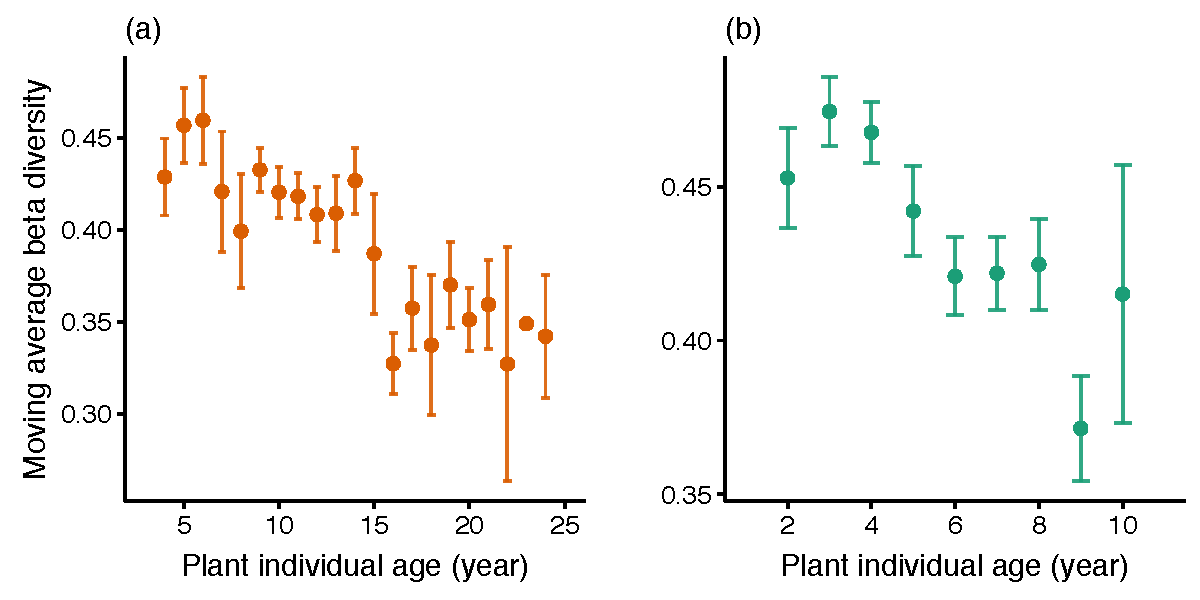
\includegraphics[width=15cm]{Chapter5/BetaDiversity_CompiledFull2015_Common_RevisedMS.pdf}}
	\caption[The relationship between plant age and beta diversity of fungal communities associated with chronosequence plant individuals when a three-year moving window was applied.]
		{\hspace{1mm} The relationship between plant age and beta diversity of fungal communities associated with chronosequence plant individuals.
		(a) and (b) show the pattern for microbial communities associated with \textit{C. edulis} (orange) and \textit{L. arboreus} (green), respectively.
		Points and error bars show the moving average trend (mean $\pm$ SE) when a three-year moving window was applied (i.e., the centroid was calculated using fungal communities associated with individuals of age $\tau - 1$, $\tau$, and $\tau + 1$; see main text for details). 
		Figure~\ref{fig:CombinedFull2015Beta_Individual_SI} shows similar trends when beta diversity was calculated as the distance of fungal communities to their age-specific centroid. 
		% See Fig.~\ref{fig:Full2015Beta_Sample} for the pattern when soil samples were plotted as observation units.
		} 
	\label{fig:CombinedFull2015Beta_Individual}
\end{figure}



\clearpage
\begin{figure}[h]
	\centering
	\makebox[\textwidth][c]{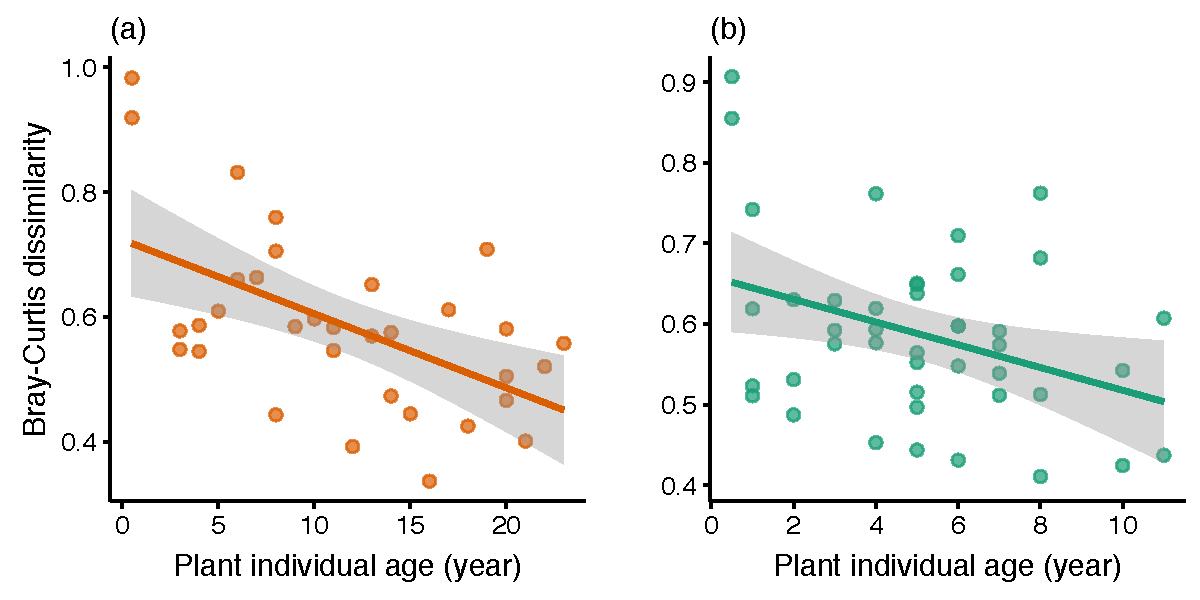
\includegraphics[width=15cm]{Chapter5/Goodness_FungiSpecies_CombinedIndividual_Full2015glmmTMBTotal_Revised2MS.pdf}}
		\caption[The relationship between plant age and Bray--Curtis dissimilarity between the fungal community observed in 2016 and the 2015 chronosequence prediction.]
		{\hspace{1mm} The relationship between plant age and Bray--Curtis dissimilarity between the fungal community observed in 2016 and the 2015 chronosequence prediction.
		(a) and (b) show the pattern for microbial communities associated with \textit{C. edulis} (orange) and \textit{L. arboreus} (green), respectively. 
		Each point represents the dissimilarity calculated for a fungal community, using samples collected in 2016 as the validation test set. See also Fig.~\ref{fig:HMSC_Species_Individual_Full2015_SI} for similar patterns when samples collected in 2017 were used as the validation test set.
		% See Fig.~\ref{fig:HMSC_Species_Sample_Full2015} or identical pattern when soil samples were plotted as observation units.
		}
	\label{fig:HMSC_Species_Individual_Full2015}
\end{figure}



\clearpage
\begin{figure}[h]
	\vspace*{-1cm}
	\centering
	\makebox[\textwidth][c]{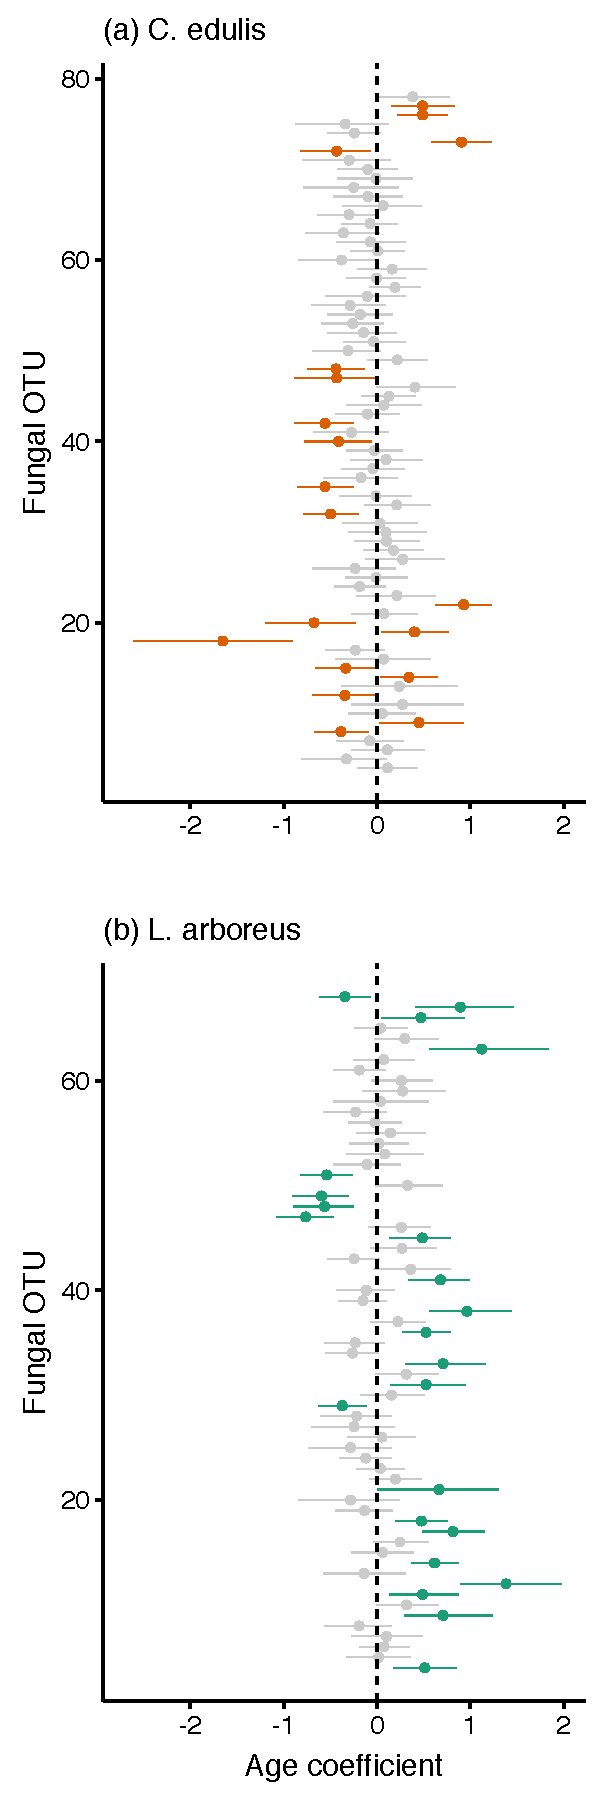
\includegraphics[width=6.5cm]{Chapter5/Funguild_HMSC_FungiSpecies_CombinedIndividual_Full2015Total_PathogenLong.pdf}}
	\caption[Predicted temporal trends of potential pathotrophic fungal OTUs associated with \textit{C. edulis} and \textit{L. arboreus} individuals.]
		{\hspace{1mm} Predicted temporal trends of potential pathotrophic fungal OTUs associated with (a) \textit{C. edulis} and (b) \textit{L. arboreus} individuals. Model fitting was performed for the two plant species separately. Points and line segments represent the mean and the 95$\%$ credible interval of the fitted age coefficient (x-axis) for different fungal OTUs (y-axis). Significant age coefficients are colored (orange for \textit{C. edulis}; green for \textit{L. arboreus}) and insignificant ones are in gray.}
		\label{fig:Funguild_HMSC_Species_Individual_Full2015Pathogen}
\end{figure}


